% Compile from this folder: pdflatex phase3_report.tex (twice).
\documentclass[11pt,a4paper]{article}

\usepackage{amsmath, amssymb, amsthm, mathtools}
\usepackage{bm}
\usepackage{graphicx}
\usepackage{tikz}
\usetikzlibrary{arrows.meta,calc,positioning,fit}
\usepackage{subcaption}
\usepackage{adjustbox}
\usepackage{booktabs}
\usepackage{tabularx}
\usepackage[numbers,sort&compress]{natbib}
\usepackage[colorlinks=true,linkcolor=blue,citecolor=blue,urlcolor=blue]{hyperref}
\usepackage[capitalise,noabbrev]{cleveref}
\usepackage{microtype}
\usepackage{parskip}
\setlength{\parindent}{0pt}
\setlength{\parskip}{6pt}
\usepackage[margin=2.5cm]{geometry}
\usepackage{xcolor}

\newcommand{\norm}[1]{\left\lVert #1 \right\rVert}
\newcommand{\Fperp}{F_{\perp}}
\newcommand{\Fpar}{F_{\parallel}}
\newcommand{\dstar}{d^{\star}}
\graphicspath{{figures/}}

\title{Sensitivity of Direct Teleoperation to Heading Error when Opening a
  Constrained Mechanism: A Simulation Study with the Franka Research 3}
\author{}
\date{}

\begin{document}
\maketitle
\vspace{-3em}

\begin{abstract}
When a robot arm holds a drawer handle, the arm and the drawer form a closed kinematic chain:
the hand can only move along the drawer's axis. Any part of a motion command that points
across the axis cannot be carried out and turns into force at the handle. This study measures
how strongly that effect limits direct teleoperation, which serves as the baseline for a
planned shared-control method. A simulated Franka Research 3 was attached to a drawer handle
in Gazebo. The task was to open the drawer by 0.25~m while keeping the sideways force at the
handle below 30~N. A scripted operator performed 48 trials with ten heading errors and three
drawer directions, each starting from a full reset. All 9 trials with a heading error of
0.25$^\circ$ or less succeeded, 2 of 6 succeeded at 0.5$^\circ$, and none of the 33 trials at
0.75$^\circ$ or more succeeded. The handle was lost after 2.7 to 5.7~mm of accumulated sideways
error. The task is therefore feasible but leaves the baseline almost no tolerance for
misalignment, which makes it a suitable test for assistance.
\end{abstract}

\section{Introduction}\label{sec:intro}

Drawers and doors can move in only one way: a drawer slides along a line and a door swings
about its hinge. Once a gripper holds the handle firmly, the arm inherits this restriction.
Motion commanded in any other direction is resisted by the mechanism and appears as force at
the handle, large enough on a real robot to pull the handle out of the gripper.

Autonomous robots deal with this by being compliant and letting the mechanism guide the hand.
Niemeyer and Slotine opened unknown doors by following the path of least resistance
\cite{niemeyer1997simple}, Jain and Kemp used equilibrium point control on a compliant arm
\cite{jain2010pulling}, and Karayiannidis et al.\ gave an adaptive controller for doors and
drawers under uncertainty \cite{karayiannidis2016adaptive}. Lutscher et al.\ estimate the
allowed direction online from the measured motion of the hand \cite{lutscher2010control}. In
teleoperation, such an estimate can drive a guidance virtual fixture
\cite{rosenberg1993virtual,marayong2003spatial}, which keeps the part of the operator's
command that points along the allowed direction and removes the rest.

To judge whether such assistance helps, three things are needed first: a repeatable task, fixed
measures of success, and a baseline that has no assistance. This study builds those three
elements and measures how the baseline fails as the operator's command turns away from the
true axis. The aim is to find the range of heading errors where the task is neither trivially
easy nor impossible, because a comparison between controllers is informative only in that range.

\section{The task}\label{sec:problem}

\Cref{fig:scene} shows the situation from above. Let $\dstar$ be the unit vector along which the
drawer opens and $F$ the force that the robot applies to the handle. The force splits into a
part along the drawer, which pulls it open, and a part across it, which the drawer resists:
\begin{equation}\label{eq:split}
  \Fpar = {\dstar}^{\top} F, \qquad
  \Fperp = F - \Fpar\, \dstar .
\end{equation}
Suppose the operator pushes in a direction that is off by a heading error $\theta$. After the
drawer has opened by $s$, the commanded position has drifted sideways from the drawer's line by
\begin{equation}\label{eq:drift}
  e_\perp = s \tan\theta .
\end{equation}
The hand cannot follow this drift, so the controller pulls towards it and $\norm{\Fperp}$ grows.
How fast it grows depends on the controller (\cref{sec:controller}).

\section{Simulation setup}\label{sec:setup}

\subsection{Environment and scene}

The experiments ran in Gazebo Classic 11 with ROS~2 Humble; joint torques are commanded through
the \texttt{ros2\_control} framework. The robot base is fixed at the origin of the world. The
drawer slides on a prismatic joint inside a fixed cabinet, and the direction it opens in is set by
the yaw angle of the cabinet. \Cref{fig:scene,fig:gui} show the scene and \cref{tab:params} lists
its parameters.

\begin{figure}[ht]
\centering
\begin{subfigure}[b]{0.48\textwidth}
  \centering
  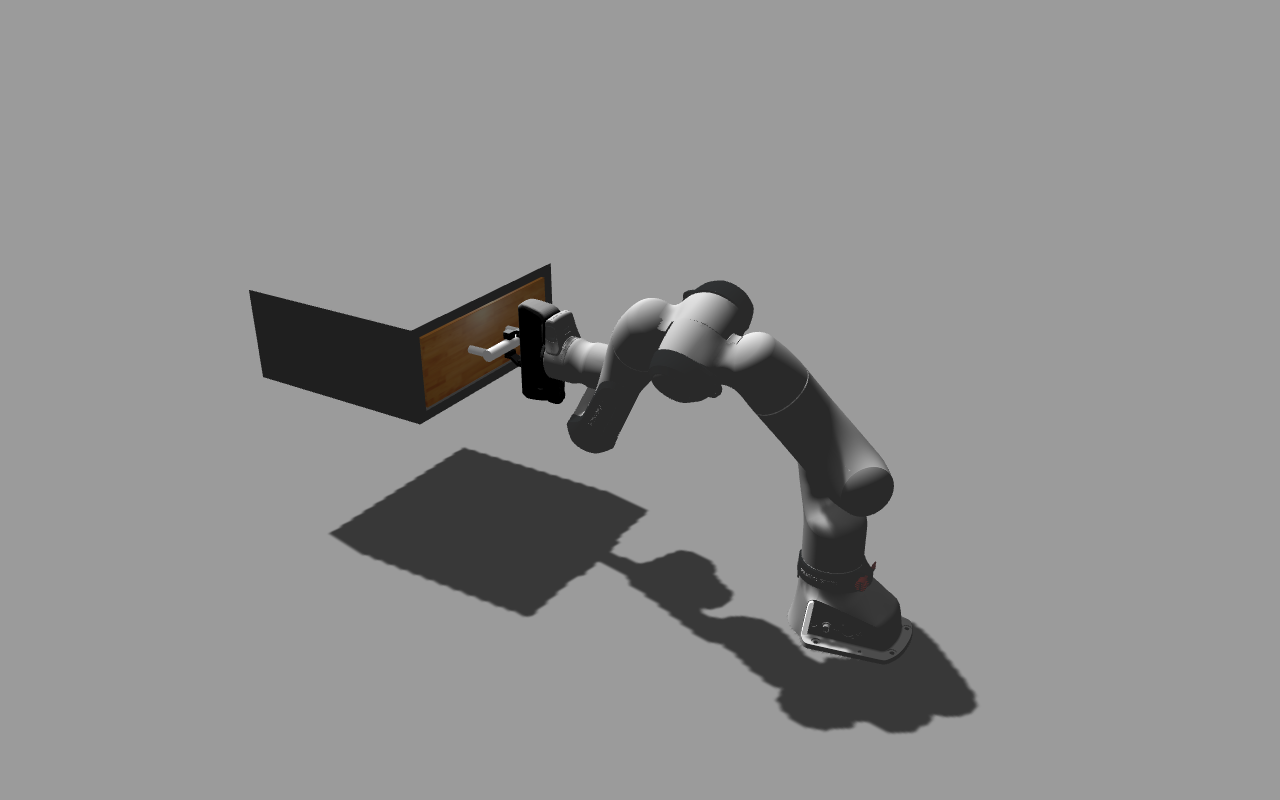
\includegraphics[width=\linewidth]{scene_start.png}
  \caption{Start of a trial, seen by the scene camera.}\label{fig:scene-shot}
\end{subfigure}\hfill
\begin{subfigure}[b]{0.48\textwidth}
  \centering
  \adjustbox{max width=\linewidth}{%
  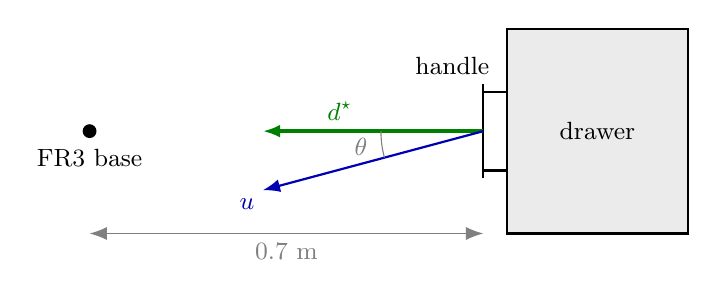
\begin{tikzpicture}[>={Latex[length=2.2mm]},font=\small]
    \fill (0,0) circle (2.5pt);
    \node[below] at (0,-0.1) {FR3 base};
    \coordinate (H) at (5,0);
    \draw[thick,fill=black!8] (5.3,-1.3) rectangle (7.6,1.3);
    \node at (6.45,0) {drawer};
    \draw[thick] (5,-0.6) -- (5,0.6);
    \draw[thick] (5,0.5) -- (5.3,0.5);
    \draw[thick] (5,-0.5) -- (5.3,-0.5);
    \node[above left] at (5.2,0.6) {handle};
    \draw[->,very thick,green!50!black] (H) -- (2.2,0) node[above,pos=0.65] {$\dstar$};
    \draw[->,thick,blue!70!black] (H) -- ++(195:2.9) node[below left=-1pt] {$u$};
    \draw[gray] (3.7,0) arc (180:195:1.3);
    \node[gray,left] at (3.65,-0.2) {$\theta$};
    \draw[<->,gray] (0,-1.3) -- (5,-1.3) node[midway,below] {0.7 m};
  \end{tikzpicture}}
  \caption{Top view. The command $u$ misses the drawer axis $\dstar$ by the heading error $\theta$.}
  \label{fig:scene-top}
\end{subfigure}
\caption{The scene: a Franka Research 3 attached to the drawer handle.}\label{fig:scene}
\end{figure}

\begin{figure}[ht]
\centering
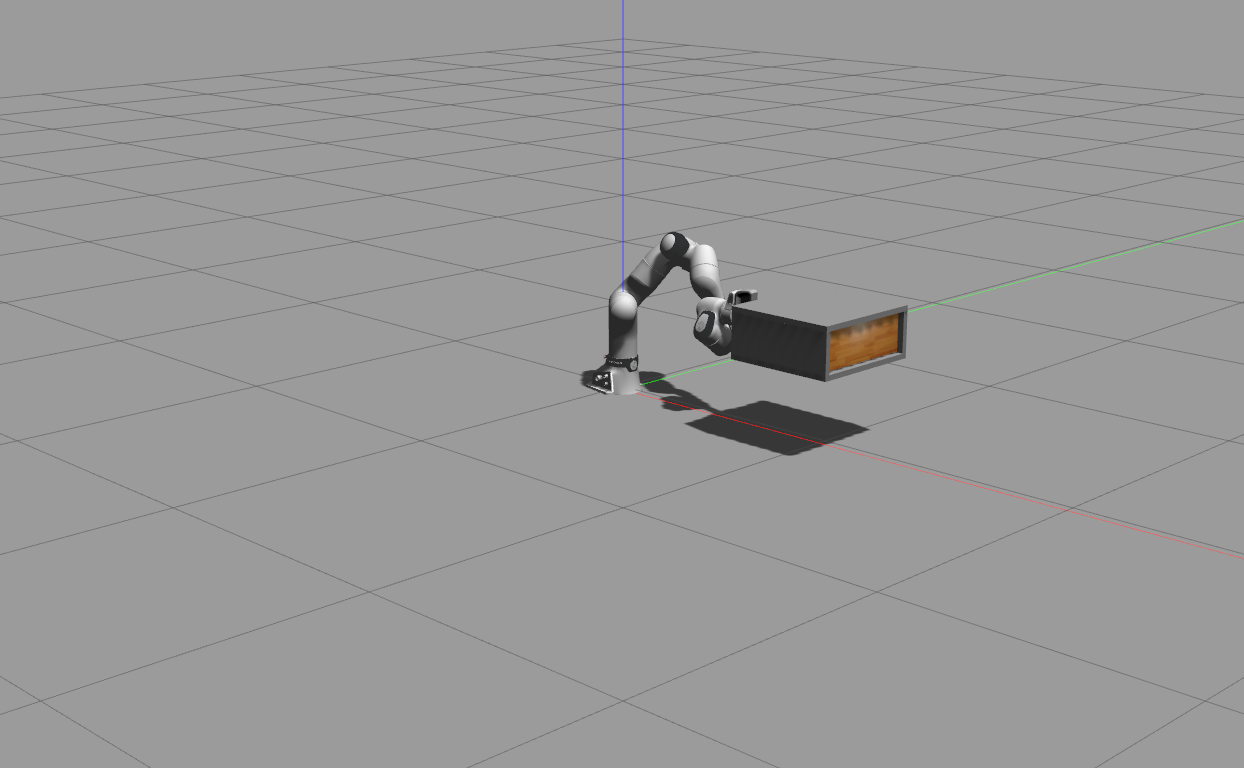
\includegraphics[width=0.65\textwidth]{gazebo_window.png}
\caption{Gazebo window (cropped) with the robot attached to the handle of the closed drawer.}
\label{fig:gui}
\end{figure}

\begin{table}[ht]
\centering
\caption{Scene parameters.}\label{tab:params}
\begin{tabularx}{\linewidth}{>{\raggedright\arraybackslash}X l}
\toprule
Parameter & Value \\
\midrule
Physics engine and step & ODE, 1~ms, real time \\
Handle position, drawer closed & $(0.7, 0, 0.4)$~m in the robot base frame \\
Drawer travel & 0 to 0.35~m \\
Drawer mass, joint damping, joint friction & 2~kg, 5~Ns/m, 3~N \\
Drawer direction & towards the robot, or tilted by $\pm 0.4$~rad \\
Grasp & rigid joint between hand and drawer \\
Robot limits & joint position and torque limits of the FR3 model \\
\bottomrule
\end{tabularx}
\end{table}

\subsection{How a trial runs}

A trial starts with the drawer closed and the centre of the gripper on the handle bar. The gripper
points into the drawer and its fingers close vertically around the bar. An inverse kinematics
search chooses the arm configuration that can follow the drawer over the required distance; for
the straight drawer it is $q_{\mathrm{arm}} = (0.788, 0.675, -1.001, -2.111, -0.097, 4.142,
-0.177)$~rad.

The trial then runs in five stages. (1)~The simulation starts paused with the arm already in this
configuration. (2)~The controllers are loaded, and physics and controllers start in the same
instant, so the arm has no time to sag. (3)~The arm settles to within 2~mrad of the start
configuration, and a rigid joint is created between hand and drawer. (4)~The arm holds still for
2~s while the command connection is established. (5)~The trial clock starts and the operator
commands motion.

\subsection{Success, failure and reset}

A trial \emph{succeeds} when the drawer has opened by 0.25~m while the sideways force
$\norm{\Fperp}$ stayed below 30~N. It \emph{fails} when $\norm{\Fperp}$ exceeds 30~N, which is
counted as losing the handle, or when 15~s pass. Because the simulated grasp never slips, handle
loss is declared from the force alone. The 30~N limit is a design assumption: a moderate grip on
a smooth handle could plausibly hold about this much, but the value was not measured on a real
gripper. The force used for this decision is the exact simulated one with the true direction
$\dstar$, which the controller never sees. A reset stops the simulation and starts it again with
the drawer closed; it took 10.9~s on average, and every trial began from one.

\section{The controller}\label{sec:controller}

\subsection{Overview}

The baseline is \emph{direct teleoperation}: the robot does exactly what the operator commands,
with no estimate of the drawer and no assistance. \Cref{fig:loop} shows the loop. An operator
command $u$ moves a target point for the gripper, inverse kinematics turns the target into joint
angles, and a PID controller in each joint produces the motor torques. Two loops run at different
rates: the target and the inverse kinematics at 50~Hz, the joint controllers at 1~kHz.

\begin{figure}[ht]
\centering
\adjustbox{max width=\textwidth}{%
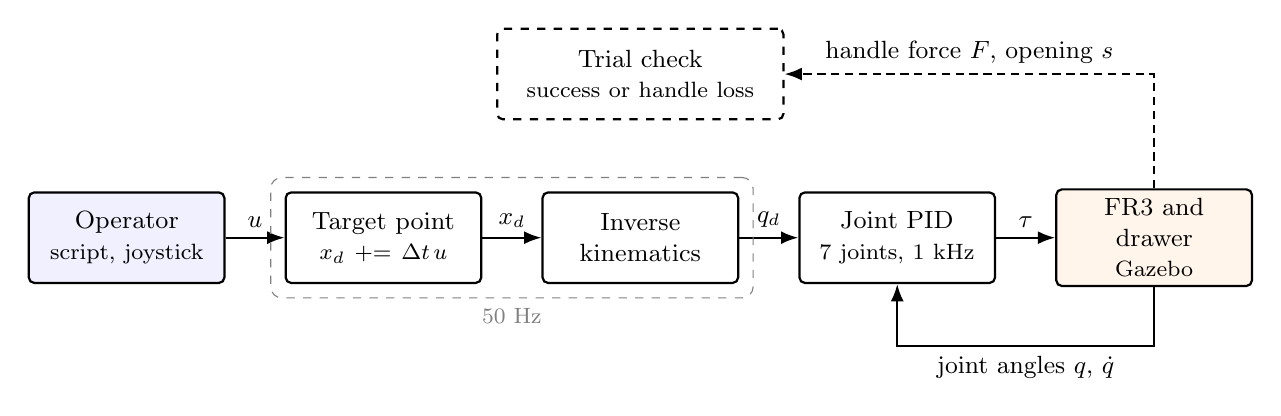
\begin{tikzpicture}[>={Latex[length=2.2mm]},font=\small,
    box/.style={draw,thick,rounded corners=2pt,align=center,minimum height=1.15cm,text width=2.25cm,fill=white},
    sig/.style={->,thick}]
  \node[box,fill=blue!6] (op) {Operator\\{\footnotesize script, joystick}};
  \node[box,right=0.75cm of op] (int) {Target point\\{\footnotesize $x_{d} \mathrel{+}= \Delta t\,u$}};
  \node[box,right=0.75cm of int] (ik) {Inverse\\kinematics};
  \node[box,right=0.75cm of ik] (pid) {Joint PID\\{\footnotesize 7 joints, 1 kHz}};
  \node[box,right=0.75cm of pid,fill=orange!8] (rob) {FR3 and drawer\\{\footnotesize Gazebo}};
  \draw[sig] (op) -- node[above] {$u$} (int);
  \draw[sig] (int) -- node[above] {$x_d$} (ik);
  \draw[sig] (ik) -- node[above] {$q_d$} (pid);
  \draw[sig] (pid) -- node[above] {$\tau$} (rob);
  \draw[sig] (rob.south) -- ++(0,-0.75) -| node[pos=0.25,below] {joint angles $q$, $\dot q$} (pid.south);
  \node[box,dashed,above=0.9cm of ik,text width=3.4cm] (chk) {Trial check\\{\footnotesize success or handle loss}};
  \draw[sig,densely dashed] (rob.north) |- node[pos=0.75,above] {handle force $F$, opening $s$} (chk.east);
  \node[draw,dashed,gray,rounded corners,fit=(int)(ik),inner sep=5pt,label={[gray,font=\footnotesize]below:50 Hz}] {};
\end{tikzpicture}}
\caption{Control loop of the baseline. Solid arrows carry commands and joint feedback. The dashed
arrow carries the measurements used only by the trial check, which ends a trial; the controller
itself never uses them.}\label{fig:loop}
\end{figure}

\subsection{Operator command}

The scripted operator used in all trials pushes at constant speed $v_{\max} = 0.1$~m/s along the
drawer direction turned horizontally by the heading error $\theta$:
\begin{equation}\label{eq:script}
  u = v_{\max}\, R_z(\theta)\, \dstar ,
\end{equation}
where $R_z(\theta)$ is a rotation about the vertical axis. It never corrects its heading. A
joystick or keyboard can replace the script; the stick deflections $a$ and the trigger value $g
\in [0,1]$ then give
\begin{equation}\label{eq:joy}
  u = g\, v_{\max}\, \phi(a), \qquad
  \phi(a) = \begin{cases} 0, & \norm{a} \le \delta, \\[2pt]
    \dfrac{a}{\norm{a}}\,\min\!\Bigl(\dfrac{\norm{a} - \delta}{1 - \delta},\, 1\Bigr), & \norm{a} > \delta, \end{cases}
\end{equation}
with a dead-zone $\delta = 0.08$ that ignores small stick movements. The trigger acts as a safety
switch: released, $g = 0$ and the robot stays still.

\subsection{Target point}

The command is a velocity, so it is added up over time into a target position $x_d$ for the
gripper centre, every $\Delta t = 0.02$~s:
\begin{equation}\label{eq:setpoint}
  x_{d,k+1} = x_{d,k} + \Delta t\, u_k .
\end{equation}
The target orientation stays equal to the orientation at the start. This is the step where the
heading error does its damage: $x_d$ follows $u$ exactly, including the sideways part that the
drawer cannot follow, which accumulates as the drift of \cref{eq:drift}.

\subsection{Inverse kinematics}

The joint angles $q_d$ that place the gripper at $x_d$ are found by damped least squares. Each
iteration compares the current gripper pose with the target, giving a 6-dimensional error $e$
(3 position components and 3 orientation components, the latter as a rotation vector), and updates
\begin{equation}\label{eq:ik}
  \Delta q = J^{+} e + \bigl(I - J^{+} J\bigr)\, k_n (q_{\mathrm{ref}} - q), \qquad
  J^{+} = J^{\top}\bigl(J J^{\top} + \lambda^{2} I\bigr)^{-1}, \qquad
  q \leftarrow q + \eta\, \Delta q ,
\end{equation}
where $J$ is the $6 \times 7$ geometric Jacobian of the arm. The damping $\lambda = 0.01$ keeps
the step bounded near singular configurations. Because the FR3 has seven joints and the task needs
six, one direction of joint motion does not move the gripper; the second term uses it to stay close
to the previous solution $q_{\mathrm{ref}}$ with gain $k_n = 0.05$. The step size is $\eta = 0.5$,
joint limits are enforced after every step, and the search stops when the error falls below
0.1~mm and 1~mrad, or after 30 iterations. Each cycle starts from the previous solution, so a few
iterations normally suffice. If no solution is found, the trial ends.

\subsection{Joint controller}

The joint angles $q_d$ go to the standard \texttt{ros2\_control} joint trajectory controller, which
interpolates between successive targets and runs an independent PID law on each joint $i$ at
1~kHz:
\begin{equation}\label{eq:pid}
  \tau_i = k_{p,i}\, e_i + k_{i,i} \int_0^t e_i \, dt' + k_{d,i}\, \dot e_i ,
  \qquad e_i = q_{d,i} - q_i ,
\end{equation}
where $\tau_i$ is the motor torque. The integral term is limited in magnitude by a clamp. The gains
are listed in \cref{tab:gains}. The integral terms let a joint reach its target exactly even when a
steady load acts on it, and the clamps stop them from growing without bound.

\begin{table}[ht]
\centering
\caption{Gains of the joint PID controllers (\cref{eq:pid}).}\label{tab:gains}
\begin{tabular}{lcccc}
\toprule
Joints & $k_p$ [Nm/rad] & $k_i$ [Nm/(rad\,s)] & $k_d$ [Nm\,s/rad] & Integral clamp [Nm] \\
\midrule
1 to 4 & 600 & 300 & 30 & 60 \\
5 & 250 & 100 & 10 & 12 \\
6 & 150 & 100 & 10 & 12 \\
7 & 50 & 50 & 5 & 12 \\
\bottomrule
\end{tabular}
\end{table}

\textbf{Gravity.} With gravity acting on the arm, the changing gravity load alone produced up to
76~N of force at the handle with no heading error, because the integral terms adapt to it slowly.
Gravity was therefore switched off for the robot links in the simulator. This is equivalent to an
exact gravity-compensation term $\tau_g(q)$ added to \cref{eq:pid}.

\subsection{What the controller means for the handle force}

In a static situation, a joint error $\Delta q$ produces torques $\tau = K_p \Delta q$ with
$K_p = \mathrm{diag}(k_{p,i})$, and the resulting force at the gripper follows from
$\tau = J^{\top} F$. Ignoring the integral and derivative terms, the arm then behaves like a spring
with compliance
\begin{equation}\label{eq:compliance}
  C = J\, K_p^{-1} J^{\top}, \qquad \delta x = C\, F .
\end{equation}
At the start configuration the proportional gains alone give a stiffness of 8.6~N/mm along the
drawer, 0.6~N/mm sideways and 0.9~N/mm vertically. The integral terms add to this: while an error
persists, they keep increasing the torque, so the force at a given error grows with time instead
of settling. In the trials, 30~N was reached after only 2.7 to 5.7~mm of sideways error, far less
than the 33 to 50~mm the proportional terms alone would require. The integral action is the most
likely explanation for this difference, although the two effects were not separated
experimentally.

\section{Sensing}\label{sec:sensing}

\textbf{Handle force.} The rigid joint that attaches the hand to the drawer reports the force it
transmits. Gazebo returns the force that the drawer applies on this joint, $f_2$, in the drawer's
own frame; the force of the robot on the handle in the robot base frame is therefore
\begin{equation}\label{eq:weld}
  F = -R_{\mathrm{drawer}}\, f_2 ,
\end{equation}
where $R_{\mathrm{drawer}}$ is the drawer's orientation. It is published at 500~Hz and smoothed with
a first-order filter of 50~ms time constant,
\begin{equation}\label{eq:filter}
  \bar F_k = \bar F_{k-1} + \alpha \bigl(F_k - \bar F_{k-1}\bigr), \qquad
  \alpha = \frac{0.002}{0.05 + 0.002} \approx 0.038 ,
\end{equation}
before it is split with \cref{eq:split} and compared with the 30~N limit. This is an exact
simulated measurement, used to score the trials.

\textbf{Joint angles and velocities} come from the simulated joint encoders and feed the inverse
kinematics and the PID controllers. \textbf{Drawer opening} $s$ is read from the drawer joint and
is used only to detect success. \textbf{A fixed scene camera} provides the operator's view and the
images in this report.

\textbf{Force from joint torques.} The physical FR3 has no force sensor at the wrist. It estimates
the force at the hand from the torque sensors in its seven joints, by subtracting the torques
that its dynamic model explains and mapping the remainder through the Jacobian. To check that a
controller could rely on this kind of estimate, the same mapping was applied to the simulated
joint torques. With the arm held still and gravity compensated,
\begin{equation}\label{eq:estimate}
  \hat F \approx \bigl(J^{\top}\bigr)^{+} \tau .
\end{equation}
For a 10~N push on the drawer, $\hat F$ changed by 11.0~N along the drawer, against 10.9~N from
the rigid joint; for a 20~N push, by 20.7~N against 22.1~N (\cref{tab:validation}). The estimate is
close while the arm is still, but this check used the commanded torques, ignored the arm's
inertia and friction, and had no sensor noise, so it does not show how well the estimate works
during motion. It was not used in the trials.

\section{Validation of the scene}\label{sec:validation}

Before the experiment, the force signal and the closed chain were checked. A known force was
applied to the drawer joint while the arm held still, and the arm was then driven along the true
path with and without a horizontal error that grew to 10~mm. \Cref{tab:validation,fig:validation}
give the results. Both mechanisms followed the arm to within 1~mm or 0.001~rad, and the injected
error increased the mean horizontal sideways force by a factor of about 70. A door was validated
as well for later use; the baseline itself was applied only to the drawer, because a fixed hand
orientation cannot follow a door as it swings.

\begin{table}[ht]
\centering
\caption{Scene validation. Sideways force is the mean horizontal $\norm{\Fperp}$.}
\label{tab:validation}
\begin{tabular}{lll}
\toprule
Check & Drawer & Door ($r = 0.6$ m) \\
\midrule
Gripper centre to handle & 0.4 mm & 0.2 mm \\
Rigid-joint reading for a 10 N (10 Nm) push & $-10.9$ N & $-6.9$ Nm about the hinge \\
Expected (friction may carry up to 3) & $-10$ to $-7$ N & $-10$ to $-7$ Nm \\
Joint-torque estimate of the same push & 11.0 N & not tested \\
Arm driven along the true path & 0.200 of 0.200 m & 0.601 of 0.600 rad \\
Sideways force on the true path & 1.2 N & 3.6 N \\
Sideways force with 10 mm of error & 87 N & 271 N \\
\bottomrule
\end{tabular}
\end{table}

\begin{figure}[ht]
\centering
\begin{subfigure}{\textwidth}
  \centering
  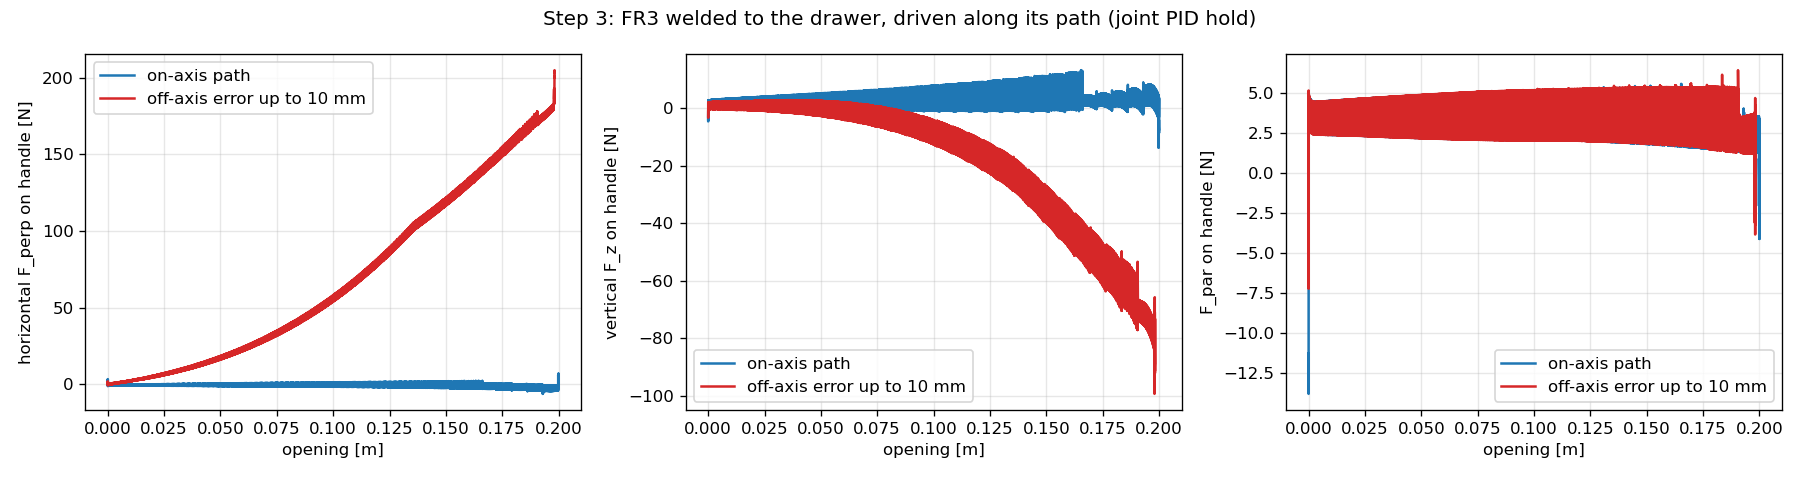
\includegraphics[width=\linewidth]{validation_drawer.png}
  \caption{Drawer.}
\end{subfigure}

\begin{subfigure}{\textwidth}
  \centering
  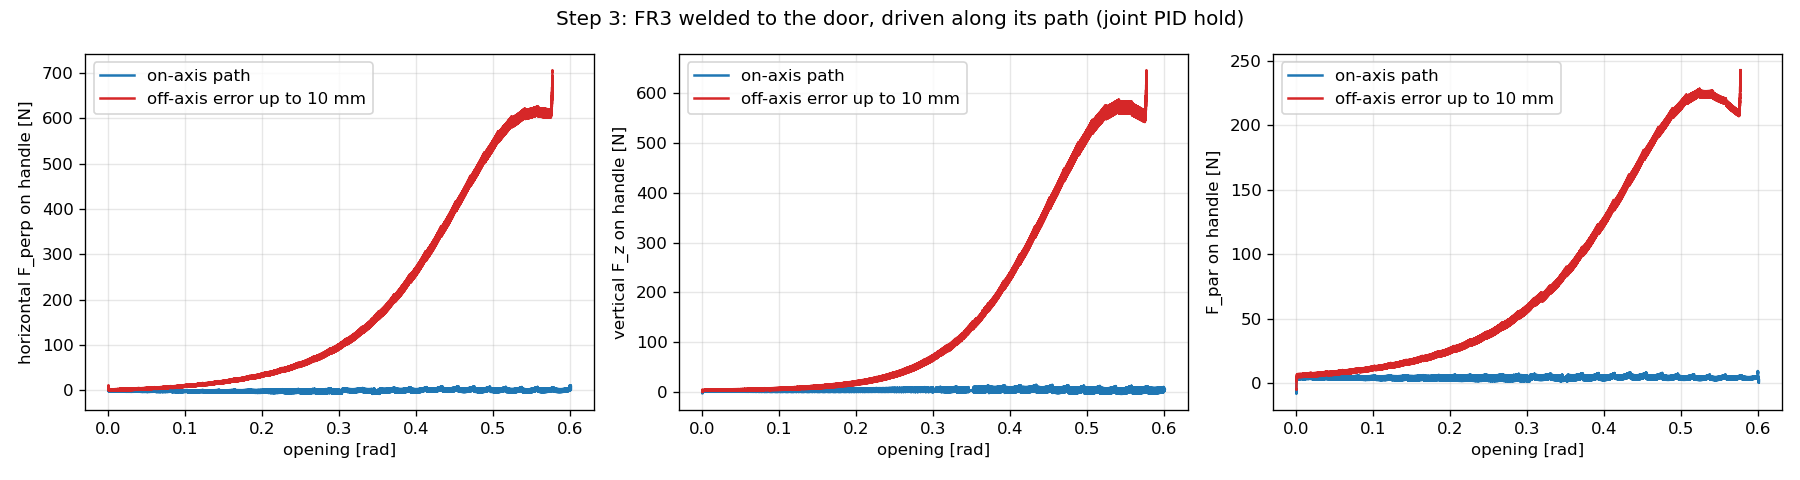
\includegraphics[width=\linewidth]{validation_door.png}
  \caption{Door.}
\end{subfigure}
\caption{Validation drives along the path, with and without a horizontal error that grows to
10~mm. From left: horizontal sideways force, vertical force, force along the path.}
\label{fig:validation}
\end{figure}

\section{Experimental design}\label{sec:design}

The heading error took ten values from 0$^\circ$ to 20$^\circ$ and the drawer direction three
values, giving 30 conditions (\cref{fig:variants}). Six conditions on the straight drawer were
repeated to four trials each, for 48 trials in total. A first run of the study was discarded
because commands were lost before the command connection was established, which caused false
early failures; the 2~s wait before each trial was added and all 48 trials were run again.

\begin{figure}[ht]
\centering
\begin{subfigure}[b]{0.48\textwidth}
  \centering
  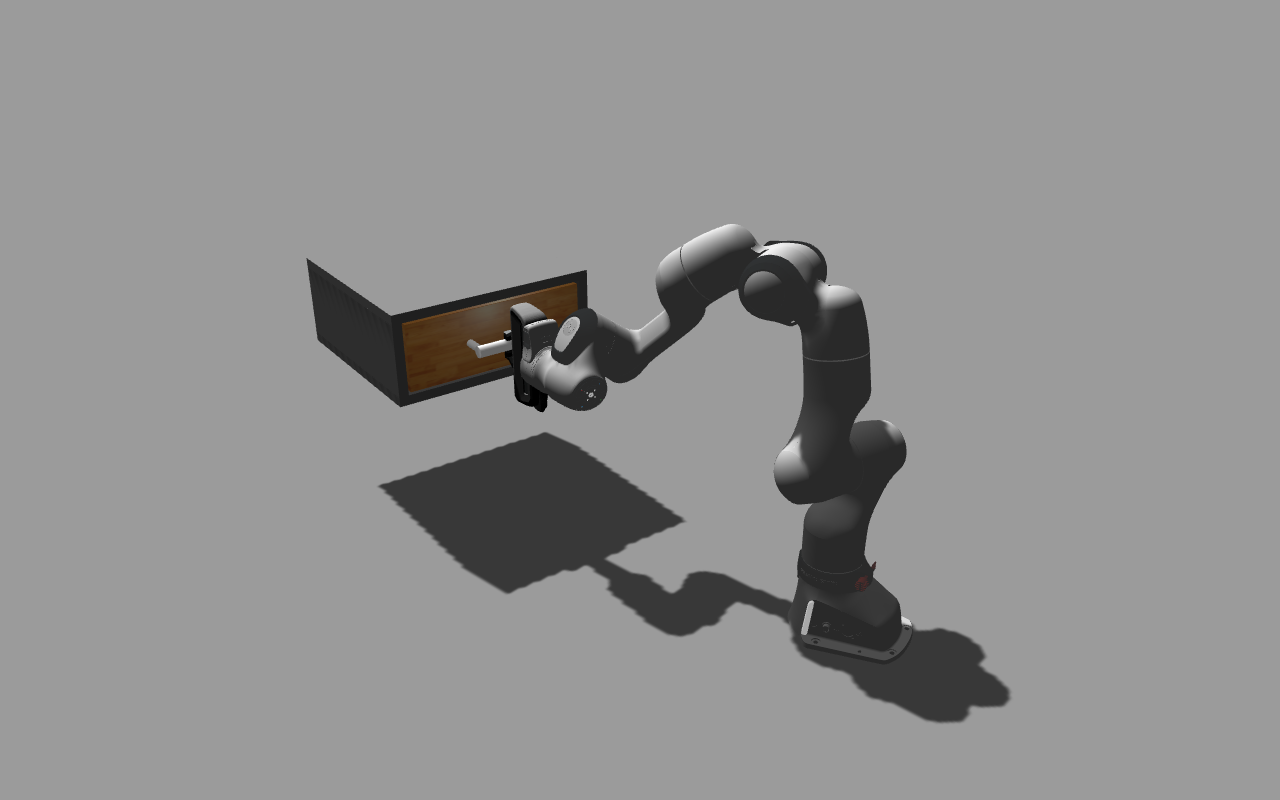
\includegraphics[width=\linewidth]{scene_tilted.png}
  \caption{Drawer direction tilted by $-0.4$~rad.}\label{fig:variant-tilted}
\end{subfigure}\hfill
\begin{subfigure}[b]{0.48\textwidth}
  \centering
  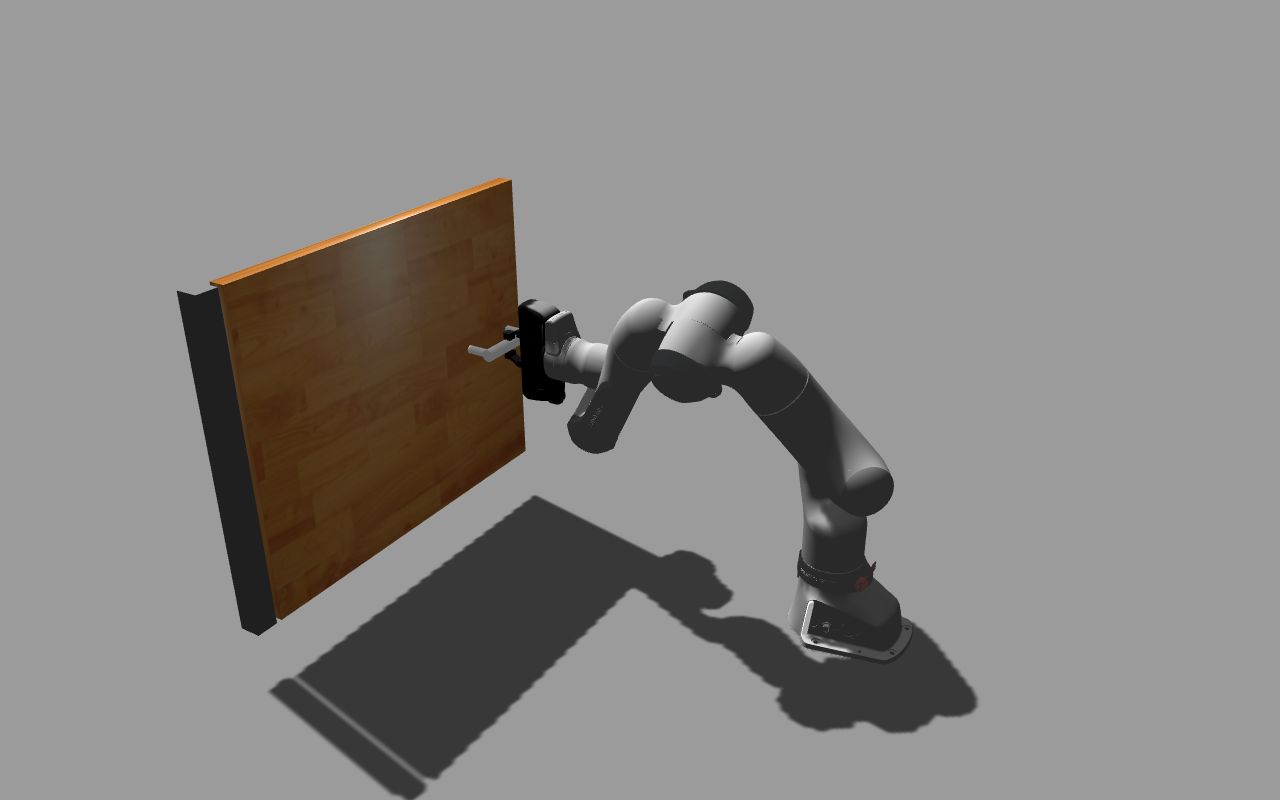
\includegraphics[width=\linewidth]{scene_door.png}
  \caption{Door, radius 0.6~m, used for validation only.}\label{fig:variant-door}
\end{subfigure}
\caption{Scene variants.}\label{fig:variants}
\end{figure}

\section{Results}\label{sec:results}

\Cref{tab:pilot,fig:outcomes} give the outcomes: 11 trials succeeded and 37 ended with the handle
lost. All 9 trials at 0.25$^\circ$ or less reached the target, in 2.56~s. At 0.5$^\circ$ the outcome
depended on the drawer direction: both tilted drawers were opened, while all four straight
trials failed. From 0.75$^\circ$ upwards all 33 trials failed. The opening reached fell steadily as
the heading error grew, from about 0.20~m at 0.75$^\circ$ to about 0.02~m at 20$^\circ$.

\begin{table}[ht]
\centering
\caption{Results by heading error. Opening is in metres, as mean $\pm$ standard deviation where
four trials were run. The last column is the largest peak sideways force in the row. Success
requires 0.25~m.}\label{tab:pilot}
\begin{tabularx}{\linewidth}{c c *{3}{>{\centering\arraybackslash}X} c}
\toprule
$\theta$ [deg] & Success & Tilt $-0.4$ rad & Straight & Tilt $+0.4$ rad & Peak $\norm{\Fperp}$ [N] \\
\midrule
% Table rows only: this fragment is \input by phase3_report.tex and does not compile alone.
0 & 6/6 & $0.251$ & $0.251 \pm 0.000$ & $0.251$ & $9.0$ \\
0.25 & 3/3 & $0.251$ & $0.252$ & $0.251$ & $21.6$ \\
0.5 & 2/6 & $0.251$ & $0.225 \pm 0.008$ & $0.250$ & $30.9$ \\
0.75 & 0/6 & $0.200$ & $0.203 \pm 0.004$ & $0.224$ & $30.7$ \\
1 & 0/3 & $0.173$ & $0.170$ & $0.194$ & $30.4$ \\
2 & 0/6 & $0.129$ & $0.110 \pm 0.000$ & $0.126$ & $30.7$ \\
3 & 0/6 & $0.095$ & $0.082 \pm 0.001$ & $0.094$ & $31.4$ \\
5 & 0/6 & $0.061$ & $0.055 \pm 0.000$ & $0.064$ & $31.0$ \\
10 & 0/3 & $0.037$ & $0.031$ & $0.036$ & $32.3$ \\
20 & 0/3 & $0.020$ & $0.016$ & $0.017$ & $33.9$ \\

\bottomrule
\end{tabularx}
\end{table}

\begin{figure}[ht]
\centering
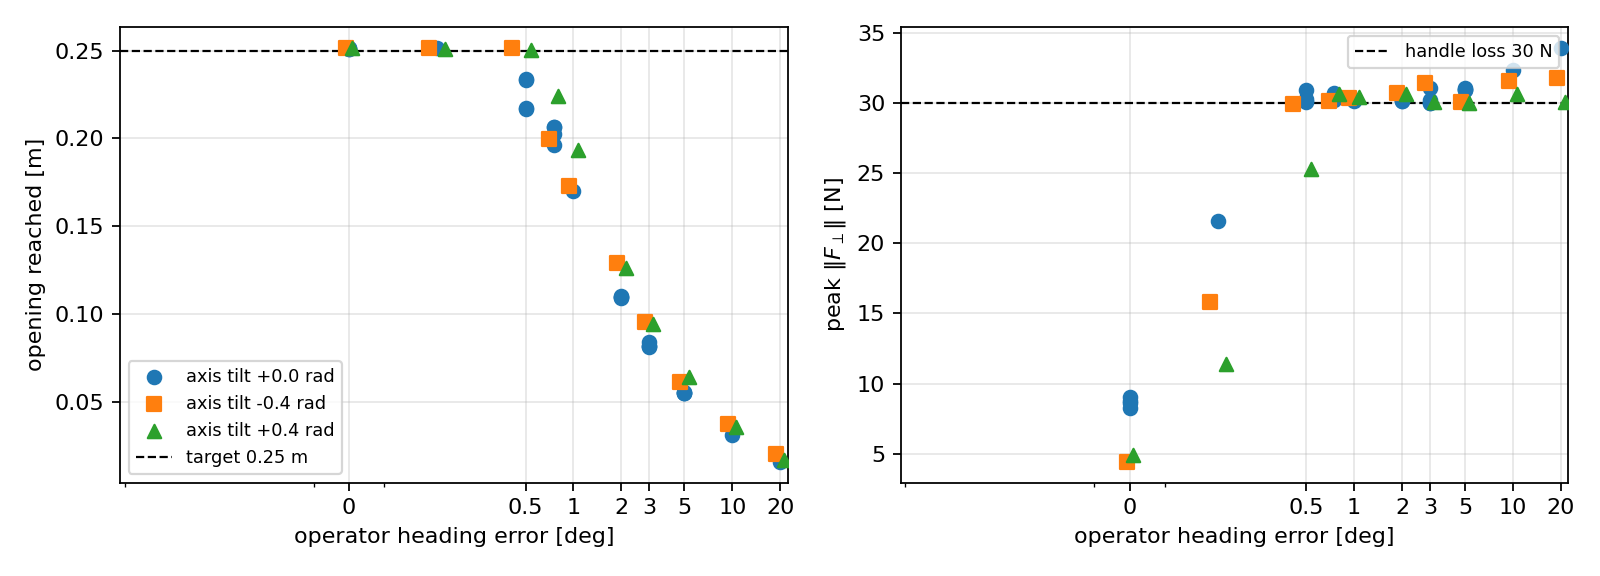
\includegraphics[width=\textwidth]{pilot_outcomes.png}
\caption{All 48 trials. Left: opening reached. Right: peak sideways force. The heading axis is
linear below 0.5$^\circ$ and logarithmic above.}\label{fig:outcomes}
\end{figure}

\Cref{fig:traces} shows how the trials fail. The drawer opens at nearly the same rate in every
trial, because it follows the arm along its axis. The trials differ in the sideways force, which
grows as the sideways error accumulates. Using \cref{eq:drift} at the moment the handle was lost,
the sideways error on the straight drawer was 2.7~mm at 0.75$^\circ$, rising to 5.7~mm at
20$^\circ$. \Cref{fig:clips} shows the end of a successful and of a failed trial.

\begin{figure}[ht]
\centering
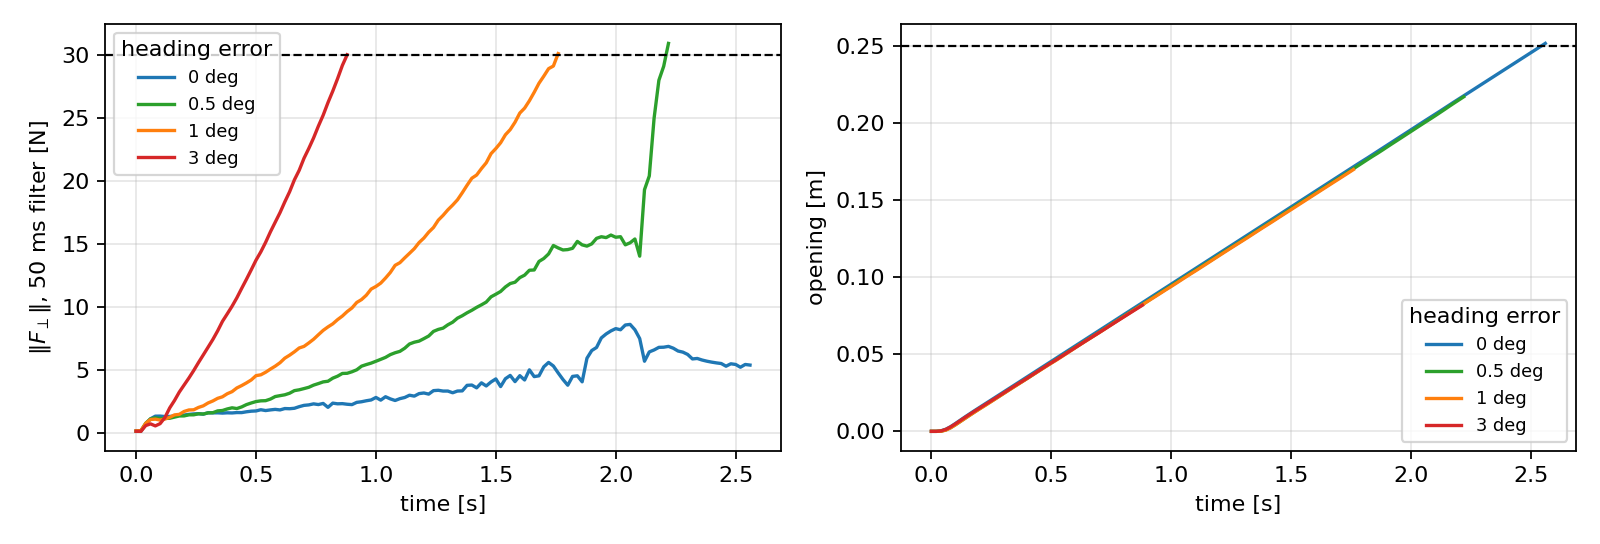
\includegraphics[width=\textwidth]{pilot_traces.png}
\caption{Straight drawer. Left: sideways force, with the 30~N limit dashed. Right: opening, with
the target dashed.}\label{fig:traces}
\end{figure}

\begin{figure}[ht]
\centering
\begin{subfigure}[b]{0.48\textwidth}
  \centering
  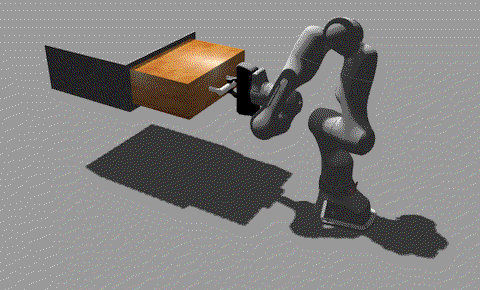
\includegraphics[width=\linewidth]{baseline_success.png}
  \caption{$\theta = 0^\circ$: target reached.}
\end{subfigure}\hfill
\begin{subfigure}[b]{0.48\textwidth}
  \centering
  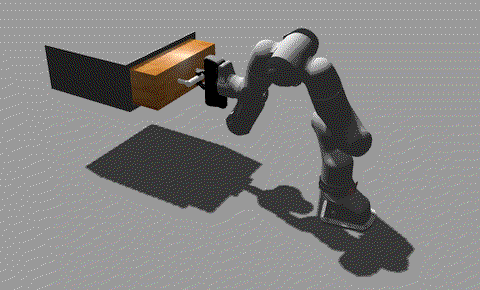
\includegraphics[width=\linewidth]{baseline_failure.png}
  \caption{$\theta = 2^\circ$: handle lost at 0.11~m.}
\end{subfigure}
\caption{End of a successful and of a failed trial.}\label{fig:clips}
\end{figure}

Repeated trials gave openings within 1~mm of each other at 0$^\circ$, 2$^\circ$ and 5$^\circ$ and
within 2.6~mm at 3$^\circ$. Near the failure boundary the spread grew to 10~mm at 0.75$^\circ$ and
17~mm at 0.5$^\circ$, so the simulation is repeatable, but not exactly so in that range.

\section{Discussion}\label{sec:discussion}

The task is feasible, since the baseline succeeds repeatably when the command is well aligned. It
is not trivial, since a 0.75$^\circ$ error already fails. An error of that size is expected to be
hard to avoid with a thumbstick, although no human operator has tried the task yet. The failures
come from the sideways part of the command, which is exactly the part that a guidance fixture
removes, so the scenario is suited to testing assistance.

The controller sets where the boundary lies. \Cref{sec:controller} showed that the joint
controllers' integral terms most likely make the force grow with time for a given error. A
Cartesian impedance controller \cite{hogan1985impedance,khatib1987unified} has no such term: its
force stays proportional to the error, at a chosen stiffness. At 400~N/m, for example, a 30~N limit
would correspond to 75~mm of error instead of a few millimetres. Direct teleoperation on such a
controller should therefore tolerate much larger heading errors. This is an estimate, and the
experiment has to be repeated with that controller.

\textbf{Limitations.}
\begin{itemize}
\item No human operator took part, and the scripted operator never corrects its heading, so the
  results do not describe human performance.
\item The gravity compensation is exact, which a real robot cannot achieve.
\item The 30~N limit is assumed, and one threshold is used for every sideways direction. A real
  gripper resists a force pressing into a finger much better than one sliding along the bar.
\item The rigid joint reported 10.9 to 11.9~N for a 10~N push in five readings. The independent
  joint-torque estimate showed the same excess for one of them (11.0~N against 10.9~N), so the
  extra force is most likely real force on the handle rather than a sensor error; its source,
  possibly the drawer's 3~N joint friction acting while the joint controllers settle, was not
  identified. Near the 30~N limit it could shift a borderline outcome.
\item In the 0.5$^\circ$ straight trials the force jumps abruptly near 0.20~m of opening
  (\cref{fig:traces}), with a smaller bump at 0$^\circ$. This is unexplained and may account for the
  difference between straight and tilted drawers at that heading.
\item Most tilted conditions were run once, so their spread is unknown.
\end{itemize}

\section{Conclusion}\label{sec:conclusion}

A repeatable simulation of a robot opening a drawer it is attached to was built, together with a
direct teleoperation baseline: the operator's velocity is added up into a target point, inverse
kinematics turns it into joint angles, and PID controllers drive the joints. The baseline
succeeded with heading errors up to 0.25$^\circ$ and failed from 0.75$^\circ$ upwards, after only a
few millimetres of sideways error, and the sideways force was the cause of every failure. The
next steps are a Cartesian impedance controller, a repeat of this study with it and with human
operators, and then online estimation of the drawer direction with guidance assistance, all
under the same task and measures.

\begin{thebibliography}{9}

\bibitem[Hogan(1985)]{hogan1985impedance}
N.~Hogan,
``Impedance control: An approach to manipulation: Part I, Theory,''
\textit{ASME Journal of Dynamic Systems, Measurement, and Control},
vol.~107, no.~1, pp.~1--7, 1985.

\bibitem[Jain and Kemp(2010)]{jain2010pulling}
A.~Jain and C.~C.~Kemp,
``Pulling open doors and drawers: Coordinating an omni-directional base and a compliant arm with
equilibrium point control,''
in \textit{Proceedings of the IEEE International Conference on Robotics and Automation (ICRA)},
2010.

\bibitem[Karayiannidis et~al.(2016)]{karayiannidis2016adaptive}
Y.~Karayiannidis, C.~Smith, F.~E.~Vi\~{n}a Barrientos, P.~\"{O}gren, and D.~Kragic,
``An adaptive control approach for opening doors and drawers under uncertainties,''
\textit{IEEE Transactions on Robotics},
vol.~32, no.~1, pp.~161--175, 2016.

\bibitem[Khatib(1987)]{khatib1987unified}
O.~Khatib,
``A unified approach for motion and force control of robot manipulators: The operational
space formulation,''
\textit{IEEE Journal on Robotics and Automation},
vol.~3, no.~1, pp.~43--53, 1987.

\bibitem[Lutscher et~al.(2010)]{lutscher2010control}
E.~Lutscher, M.~Lawitzky, G.~Cheng, and S.~Hirche,
``A control strategy for operating unknown constrained mechanisms,''
in \textit{Proceedings of the IEEE International Conference on Robotics and Automation (ICRA)},
Anchorage, AK, USA, 2010.

\bibitem[Marayong et~al.(2003)]{marayong2003spatial}
P.~Marayong, M.~Li, A.~M.~Okamura, and G.~D.~Hager,
``Spatial motion constraints: Theory and demonstrations for robot guidance using virtual
fixtures,''
in \textit{Proceedings of the IEEE International Conference on Robotics and Automation (ICRA)},
2003.

\bibitem[Niemeyer and Slotine(1997)]{niemeyer1997simple}
G.~Niemeyer and J.-J.~E.~Slotine,
``A simple strategy for opening an unknown door,''
in \textit{Proceedings of the IEEE International Conference on Robotics and Automation (ICRA)},
1997, pp.~1448--1453.

\bibitem[Rosenberg(1993)]{rosenberg1993virtual}
L.~B.~Rosenberg,
``Virtual fixtures: Perceptual tools for telerobotic manipulation,''
in \textit{Proceedings of the IEEE Virtual Reality Annual International Symposium (VRAIS)},
1993.

\end{thebibliography}

\end{document}
